% ======================================================================
%  Compile with XeLaTeX (required for the Arabic text on the page de
%  garde and for using Times New Roman as a system font):
%
%       xelatex main.tex
%       biber main
%       xelatex main.tex
%       xelatex main.tex      (run again so citations/ToC/LoF are correct)
%
% ======================================================================

\documentclass[12pt, a4paper]{report}

\usepackage[a4paper, left=2.5cm, right=2.5cm, top=2.5cm, bottom=2.5cm,
            includefoot, footskip=1.25cm]{geometry}

\usepackage{fontspec}
\setmainfont{TeX Gyre Termes}

\usepackage{polyglossia}
\setmainlanguage{english}
\setotherlanguage{french}
\setotherlanguage{arabic}
\newfontfamily\arabicfont[Script=Arabic]{Amiri}


\usepackage{setspace}
\onehalfspacing
\usepackage{parskip}          % 6pt space after paragraphs
\setlength{\parindent}{1.25cm} % retrait en début de paragraphe


\usepackage{titlesec}
\setcounter{secnumdepth}{3}
\setcounter{tocdepth}{3}

\titlespacing*{\chapter}{0pt}{0pt}{12pt}
\titlespacing*{\section}{0pt}{12pt}{6pt}
\titlespacing*{\subsection}{0pt}{12pt}{6pt}
\titlespacing*{\subsubsection}{0pt}{12pt}{6pt}

\usepackage{graphicx}
\graphicspath{{images/}}
\usepackage{float}
\usepackage{caption}
\usepackage{booktabs}
\usepackage{tabularx}
\usepackage[hidelinks]{hyperref}
\usepackage{listings}
\lstdefinelanguage{SPARQL}{
  morekeywords={SELECT,DISTINCT,WHERE,FILTER,OPTIONAL,UNION,ORDER,BY,
    DESC,ASC,LIMIT,GROUP,HAVING,COUNT,COALESCE,AS,NOT,EXISTS,
    BIND,CONSTRUCT,INSERT,VALUES,PREFIX,STRLEN,STR,STRSTARTS,IN,
    FILTER,GROUP_CONCAT},
  sensitive=false,
  morecomment=[l]{\#},
  morestring=[b]",
}
\lstset{
  basicstyle=\small\ttfamily,
  breaklines=true,
  frame=single,
  numbers=left,
  numberstyle=\tiny,
  captionpos=b,
  language=SPARQL,
}

\usepackage{fancyhdr}
\pagestyle{fancy}
\fancyhf{}
\fancyfoot[R]{\thepage}
\renewcommand{\headrulewidth}{0pt}
\fancypagestyle{plain}{%
  \fancyhf{}
  \fancyfoot[R]{\thepage}
  \renewcommand{\headrulewidth}{0pt}
}
\usepackage[citestyle=numeric, bibstyle=numeric, sorting=none, backend=biber]{biblatex}
\addbibresource{references.bib}

\begin{document}

\pagestyle{empty}
% ======================================================================
%  This file is \input from main.tex — do not compile it standalone.
% ======================================================================
\begin{titlepage}
\begin{french} % whole page de garde stays French, even though the
               % rest of the report body is written in English
\centering

{\small République Algérienne Démocratique et Populaire}\\
\begin{Arabic}
الجمهورية الجزائرية الديمقراطية الشعبية \\
\end{Arabic}
{\small Ministère de l'Enseignement Supérieur et de la Recherche Scientifique}\\
\begin{Arabic}
وزارة التعليم العالي و البحث العلمي \\
\end{Arabic}

\rule{\linewidth}{0.3mm} \\[0.4cm]

\begin{minipage}{5cm}
    \begin{center}
        
\includegraphics[width=5cm]{esi_logo.png}
    \end{center}
\end{minipage}\hfill
\begin{minipage}{10cm}
    \begin{flushright}
    \begin{Arabic}
    المدرسة الوطنية العليا للإعلام الآلي \\
    (المعهد الوطني للتكوين في الإعلام الآلي سابقا)
    \end{Arabic}\\
    {\small École nationale Supérieure d'Informatique}\\[0.1cm]
    {\small ex. INI (Institut National de formation en Informatique)}\\[0.1cm]
    \end{flushright}
\end{minipage}\hfill\\

\rule{\linewidth}{0.3mm} \\[1cm]


% -------------------------------------------------------------
% Titre du rapport — Annexe 2
% -------------------------------------------------------------
{\Large\bfseries Rapport de stage (SPE)}\\[0.3cm]
{\large 2\textsuperscript{ème} année Cycle Supérieur (2CS)}\\[1cm]

% -------------------------------------------------------------
% -------------------------------------------------------------
{\large Option~: Systèmes Informatiques (SQ)\\}
\vspace{1cm}

% -------------------------------------------------------------
% Thème — Annexe 2
% -------------------------------------------------------------
\begin{center}

\begin{minipage}{0.9\linewidth}
\centering
{\Large \textbf{Thème :}\par}
{\Large\bfseries Enterprise Architecture Knowledge Graphs (EAKGs)\par}

\end{minipage}

\end{center}
\vspace{3cm}

% -------------------------------------------------------------
% Réalisé par / Encadré par — Annexe 2
% -------------------------------------------------------------
\ \begin{minipage}[t]{0.45\textwidth}
        \begin{flushleft} \large
            \textbf{Réalisé par :}\\
            \vspace{0.2cm}
            --BELGUESMIA Oussama \\
            --KHIARI Anis nassim
        \end{flushleft}
    \end{minipage}
    \hfill
    \begin{minipage}[t]{0.45\textwidth}
        \begin{flushleft} \large
            \textbf{Encadré par :}\\
            \vspace{0.2cm}
                --KHOURI Selma\\
                --SAID LHADJ Lynda
        \end{flushleft}
    \end{minipage}\par\vspace{1cm}

    \begin{flushleft} \large
        \textbf{Organisme d'accueil :} Laboratoire de la Communication dans les Systèmes Informatiques (LCSI), ESI
    \end{flushleft}

    \vfill  
    \rule{0.75\linewidth}{0.3mm} \\[0.5cm]
        {\large Année universitaire~: 2026 -- 2027}\\[1.5cm]
    
\end{french}
\end{titlepage}

\pagestyle{fancy}
\pagenumbering{roman}

\chapter*{Abstract}
\addcontentsline{toc}{chapter}{Abstract}
Enterprise architecture (EA) models provide an integrated representation of an organization's business, application, and technology layers, yet traditional modeling tools do not always make this interconnected data easy to analyze. This work presents a methodology for transforming ArchiMate models into Semantic Web Knowledge Graphs (KGs). We introduce a phased translation algorithm that converts ArchiMate Model Exchange Format (XML) into an RDF/OWL ontology. Building on this graph, we deploy a SPARQL-based analytical pipeline directly within the triplestore to support architectural evaluations, including TOGAF Gap Analysis and the detection of structural EA smells. Finally, we evaluate the use of Large Language Models (LLMs) to explore these EA models through natural language. Our experiments contrast static context provisioning (XML, JSON, and Turtle dumps) with interactive, tool-based access via GraphDB. In this setup, the interactive condition achieved a higher mean final score (0.90) than the static representations, suggesting that dynamic access to semantic graphs may be useful for AI-assisted enterprise architecture analysis.


\noindent\textbf{Keywords:} Enterprise Architecture; ArchiMate; Knowledge Graphs; RDF/OWL; Large Language Models.

\tableofcontents

\addcontentsline{toc}{chapter}{List of Figures}
\listoffigures

\addcontentsline{toc}{chapter}{List of Tables}
\listoftables

\chapter*{List of Abbreviations}
\addcontentsline{toc}{chapter}{List of Abbreviations}
\begin{description}
    \item[ABB] Architecture Building Block
    \item[API] Application Programming Interface
    \item[DBMS] Database Management System
    \item[EA] Enterprise Architecture
    \item[EAKG] Enterprise Architecture Knowledge Graph
    \item[IRI] Internationalized Resource Identifier
    \item[JSON] JavaScript Object Notation
    \item[KG] Knowledge Graph
    \item[LLM] Large Language Model
    \item[OWL] Web Ontology Language
    \item[RDF] Resource Description Framework
    \item[RDFS] RDF Schema
    \item[SPARQL] SPARQL Protocol and RDF Query Language
    \item[TOGAF] The Open Group Architecture Framework
    \item[TTL] Turtle
    \item[URI] Uniform Resource Identifier
    \item[XML] Extensible Markup Language
\end{description}


\cleardoublepage
\pagenumbering{arabic}

\chapter*{Introduction}
\addcontentsline{toc}{chapter}{Introduction}

Enterprise architecture models offer an integrated and unified representation of the different layers of an organization's activity, thereby facilitating decision-making. These layers structure the vision of business processes, application architecture, technical infrastructure, as well as the interactions between them.

Modeling languages that allow for the mapping of this architecture are widely used, such as ArchiMate, the standard language of the Open Group. However, to fully exploit these models and automate their analysis via complex queries, a transition to Knowledge Graphs (KG) is being adopted \parencite{glaser2022model}. KGs are currently deployed on a large scale, ranging from the massive KGs of web giants (Google, Facebook, or Amazon) to more targeted enterprise KGs.

Tools like the EAKG Toolkit \parencite{glaser2022toolkit} allow ArchiMate models to be transformed into a KG based on the Property Graph model (supported by the Neo4j DBMS). Another KG standard, originating from the Semantic Web, is the RDF graph model (supported by other DBMSs such as GraphDB).

The objective of this project is to:
\begin{enumerate}
    \item Provide an algorithm allowing the translation of an ArchiMate model according to the RDF standard. Examples of ArchiMate models are provided as input (in XML). The algorithm, inspired by prior work \parencite{glaser2022model}, must provide the RDF representation of these models. The user will thus be able to export the resulting RDF KG to a DBMS of their choice (GraphDB in our case).
    \item Propose queries to analyze ArchiMate models through the KG. The queries will be formulated in SPARQL, the standard language for querying the RDF model, similar to SQL for querying a relational model.
    \item The use of an LLM can be considered to allow querying the obtained KG in natural language---English---(translating the natural language query into the SPARQL language).
\end{enumerate}

\chapter{Translation Methodology: ArchiMate to RDF/OWL}
\label{chap:translation}

This chapter presents the methodology adopted for translating an ArchiMate model to RDF Knowledge Graphs, and designing an OWL ontology\parencite{w3c-owl} to represent ArchiMate standard semantics and allow better usability of the resulting graph. It begins with the motivation for using Knowledge Graphs in enterprise architecture management, reviews the existing EAKG Tool approach, and then details our ArchiMate-to-RDF translation rules, our Archimate ontology design, and the phased construction lifecycle.

% ------------------------------------------------------------------
\section{Knowledge Graphs for Enterprise Architecture}
\label{sec:why-kg}

EA models have a graph structure, but current analysis tools do not take full advantage of this property, which allows differentiation of relations between elements, discovery of paths, clusters, and graph metrics. Moreover, current tools offer a limited set of visualization techniques.

Knowledge Graphs ease advanced reasoning---whether rule-based or machine learning---to provide question-answering capabilities. A model-based construction method combined with graph enrichment can exploit the KG representation and reasoning \parencite{glaser2022model}. Graph visualization can be easily customized, and storing the graph in a graph database enables efficient execution of complex queries. Several graph-based methods have been proposed to analyze EA models, including failure impact analysis with Bayesian Belief Networks and fault trees to analyze the availability of EA components.

% ------------------------------------------------------------------
\section{Related Work: The EAKG Tool}
\label{sec:eakg-tool}

A model-based construction method for Enterprise Architecture Knowledge Graphs is proposed in \parencite{glaser2022model}. The approach maps ArchiMate models to a Property Graph representation, following a two-phase lifecycle:

\subsection{Creation Phase (Knowledge Extraction)}
\label{subsec:eakg-creation}

During the creation phase, ArchiMate layers and aspects are mapped to KG properties. Types (classes) are derived from the layer-specific metamodel. KG nodes and edges are derived from the concrete ArchiMate model (element names, connections). Relationships are mapped to edges, and relationship connectors are mapped to properties (AND/OR). Concrete behavioral and structural elements are mapped to nodes, while abstract details are mapped to properties (structure/behavioral element).

\subsection{Knowledge Graph Enrichment}
\label{subsec:eakg-enrichment}

In the enrichment phase, general graph characteristics are added as properties to nodes, such as centralities, communities (node colors), and node size. Each node is associated with PageRank, betweenness, degree, Louvain, label propagation, and WCC scores, which can be useful for analysis. A color is assigned to each node based on ArchiMate color conventions. Additionally, smells are detected and affected nodes are labeled.

\subsection{Knowledge Graph Deployment}
\label{subsec:eakg-deployment}

The resulting graph database (a Neo4j instance) contains the enriched graph with detected smells. The EAKG Toolkit \parencite{glaser2022toolkit} provides an implementation of this pipeline as a plugin for the Archi modeling tool.

Our equivalent mapping from ArchiMate models to RDF Knowledge Graphs is formalized later in Section~\ref{sec:rules}.

% ------------------------------------------------------------------
\section{ArchiMate to RDF: Our Approach}
\label{sec:rdf-approach}

Following the approach presented in \parencite{glaser2022model}, we translate ArchiMate models into RDF Knowledge Graphs. The detailed mapping is defined in Section~\ref{sec:rules}; Section~\ref{sec:ontology} introduces the ontology, which provides the semantic vocabulary used by those rules.

% ------------------------------------------------------------------
\section{The Base Ontology}
\label{sec:ontology}

The ArchiMate framework organizes concepts along two dimensions: \emph{layers} (Strategy, Business, Application, Technology, Physical, and Implementation \& Migration) and \emph{aspects} (Passive Structure, Behavior, Active Structure, and Motivation), as defined by the ArchiMate standard \parencite{opengroup2023archimate}. Our ontology maps the ArchiMate metamodel to OWL classes; its class hierarchy mirrors the metamodel's Layer/Aspect/Concept structure. To illustrate how the ontology classifies architecture elements, Figure~\ref{fig:businessactor-example} shows an example for \texttt{BusinessActor}.

\begin{figure}[H]
  \centering
  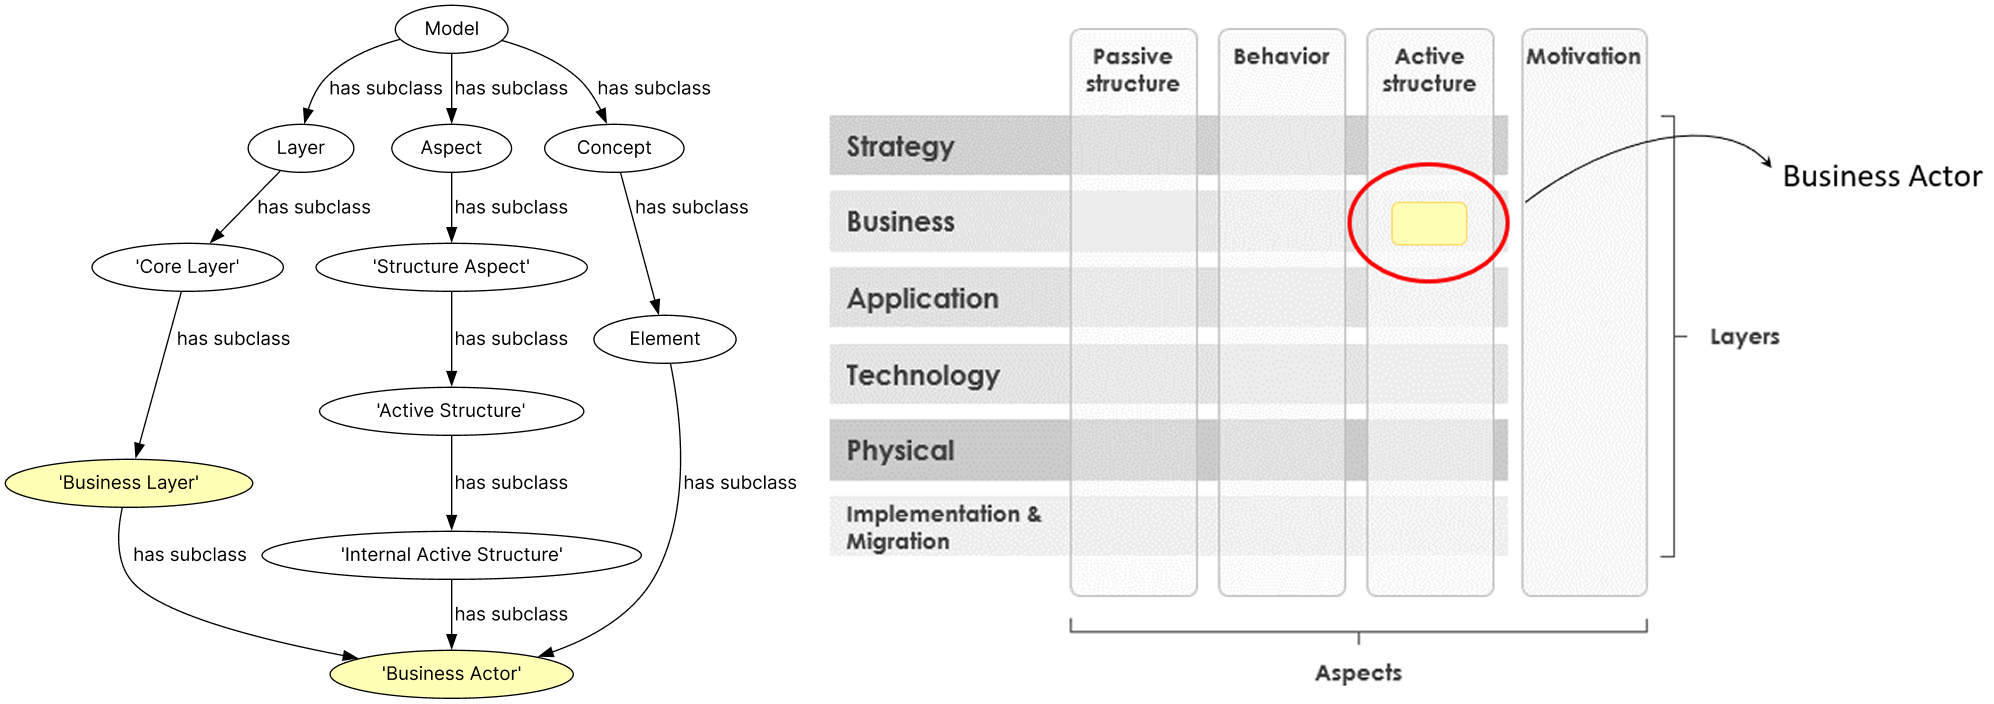
\includegraphics[width=\linewidth]{image2.png}
  \caption{Example: classification of \texttt{BusinessActor} in the ontology hierarchy and its position in the ArchiMate framework}
  \label{fig:businessactor-example}
\end{figure}

\subsection{Relationships in the Ontology}
\label{subsec:ontology-relationships}

Relationships are modeled as \texttt{owl:ObjectProperty} instances, which connect elements directly. They are organized into four base properties: \texttt{structuralRelationship}, \texttt{dependencyRelationship}, \texttt{dynamicRelationship}, and \texttt{otherRelationship}. Relationship connectors (AND, OR) are modeled as a class that is instantiated to create a junction, then assigned the type ``and'' or ``or''; elements participate in the junction through the appropriate relationship.

% ------------------------------------------------------------------
\section{ArchiMate Model Exchange Format}
\label{sec:exchange-format}

The ArchiMate Model Exchange Format stores a model in XML. The top-level model contains separate containers for the information needed by the translator, notably \texttt{<propertyDefinitions>}, \texttt{<elements>}, and \texttt{<relationships>}. Property definitions declare the available property keys and their datatypes. Element records provide identifiers, types, names, documentation, and property values, while relationship records provide identifiers, relationship types, source and target references, and any associated metadata.

The translator reads these containers in a controlled order: property definitions establish the vocabulary for custom properties, elements establish the resources and their types, and relationships connect those resources. Names and documentation may appear in language-specific \texttt{<name>} and \texttt{<documentation>} entries, so the corresponding language information is preserved when the XML is converted to RDF literals. The resulting RDF/OWL structure is specified formally in Section~\ref{sec:rules}.

% ------------------------------------------------------------------
\section{Knowledge Graph Construction Lifecycle}
\label{sec:kg-lifecycle}

To ensure modularity and extensibility, this translation algorithm formally adopts the phased Model-based Knowledge Graph Construction Process.

\subsection{Phase 1: Knowledge Graph Creation (Base Graph Construction)}
\label{subsec:phase1}

In the Knowledge Graph Creation stage, the relevant information is extracted from the EA model to establish the initial semantic topology of the EAKG. Property definitions are registered first, followed by the creation and typing of element resources and the connection of those resources through relationship predicates. The base graph is grounded using \texttt{rdf:type} and \texttt{rdfs:subPropertyOf}, defining the ArchiMate entities present and preparing the graph for enrichment. The exact representation of each resource, relationship, and property is given in Section~\ref{sec:rules}.

The canonical ArchiMate schema ontology is published at the persistent URL \texttt{http://purl.org/eakg/archimate}, which also serves as the Ontology IRI. The PURL redirects to the file's current hosting location, so identifiers stay stable even if the hosting changes. The methodology enforces a strict separation between \emph{static schema} (the published ontology, containing class hierarchies, relationship types, and schema-fixed attribute declarations) and \emph{dynamic output} (the translator, which emits only model-specific instance data such as per-relation predicates and user-defined properties).

\subsection{Phase 2: Knowledge Graph Enrichment (Semantic Layering)}
\label{subsec:phase2}

The Enrichment Phase expands the base graph with the semantic hierarchy and domain-specific analytical tags. It proceeds in two steps.

First, the ArchiMate and EA smell ontologies are loaded into the triplestore directly via their persistent URLs (\texttt{http://purl.org/eakg/archimate} and \texttt{http://purl.org/eakg/smells}), alongside the translated model. This supplies the \texttt{rdfs:subClassOf} and \texttt{rdfs:subPropertyOf} hierarchy that the base graph does not contain---for example, connecting \texttt{archimate:BusinessActor} through \texttt{archimate:ActiveStructureElement} up to \texttt{archimate:BusinessLayer}. When an RDFS ruleset is active, the triplestore expands these hierarchies automatically. No offline merge script is needed.

Second, EA smells are detected and tagged via SPARQL. For each of the seven smells defined in the smell ontology, a detection \texttt{SELECT} query identifies the affected resources, and a tagging \texttt{INSERT} query materializes a \texttt{smells:hasSmell} triple on each one. The detection queries and their tagging counterparts are presented in Chapter~\ref{chap:queries}.

This differs from the enrichment approach of \parencite{glaser2022model}, where computed graph metrics and EA smell labels are materialized by an external pipeline. Our approach performs enrichment directly in the triplestore via SPARQL updates, avoiding the need for a separate enrichment script. Structural graph analytics such as centrality scores remain a potential future extension.

% ------------------------------------------------------------------
\section{Core Translation Rules}
\label{sec:rules}

\subsection{Rule 1: Elements (Vertices)}
\label{subsec:rule1}

In the Creation Phase, an ArchiMate element represents a distinct entity in the EAKG. Specifically, this targets a concrete element of the target ArchiMate model (e.g., a Business Actor or Application Service).

\begin{itemize}
    \item Each element identifier becomes an \texttt{owl:NamedIndividual}; the element is typed with its ArchiMate class and acts as an RDF subject or object. Names and documentation become multilingual \texttt{rdfs:label} and \texttt{rdfs:comment} triples.
\end{itemize}

\subsection{Rule 2: Relations (Edges)}
\label{subsec:rule2}

ArchiMate relationships map to edges in the EAKG, acting as the semantic link between elements.

\begin{itemize}
    \item The relationship identifier becomes an \texttt{owl:ObjectProperty} used directly as the source-to-target predicate. Its optional name and documentation are attached to that predicate as multilingual \texttt{rdfs:label} and \texttt{rdfs:comment} triples. \texttt{rdfs:subPropertyOf} connects it to the corresponding ArchiMate relationship type, avoiding RDF-star reification; relationship properties are emitted as direct triples on the relationship predicate.
\end{itemize}

\subsection{Rule 3: Property Definitions and Instances}
\label{subsec:rule3}

Abstract details of elements and relations are mapped to properties of the KG metamodel \parencite{glaser2022model}. Because each property's name (key) is guaranteed unique within the ArchiMate global property manager \parencite{opengroup2019exchange}, this identity is used directly as the property's own predicate:

\begin{itemize}
    \item A property key becomes an \texttt{owl:DatatypeProperty} with an XSD range and an \texttt{rdfs:subPropertyOf} link to \texttt{archimate:Property}, even when it has no assigned value. Values are emitted as direct subject--predicate--literal triples, so repeated values remain distinct objects without intermediate nodes.
    \item \textbf{Schema-fixed attributes.} Certain relationship types carry semantic metadata as fixed XML attributes rather than \texttt{<property>} child elements---specifically \texttt{accessType} (on Access), \texttt{isDirected} (on Association), and \texttt{modifier} (on Influence). The schema declaration (type, range, super-property under \texttt{archimate:Property}) lives in the static ontology; concrete values are emitted by the translator.
\end{itemize}

\begin{lstlisting}[basicstyle=\small\ttfamily,
                    breaklines=true,
                    frame=single,
                    caption={Input ArchiMate fragment used in the worked example},
                    label={lst:worked-xml}]
<propertyDefinitions>
  <propertyDefinition identifier="propdef-1" type="string">
    <name xml:lang="en">Vendor</name>
  </propertyDefinition>
</propertyDefinitions>

<element identifier="id-47045" xsi:type="Node">
  <name xml:lang="en">Data Acquisition Gateway</name>
  <properties>
    <property propertyDefinitionRef="propdef-1">
      <value>Cisco</value>
    </property>
  </properties>
</element>
<element identifier="id-47052" xsi:type="CommunicationNetwork">
  <name xml:lang="en">Home &amp; Away LAN</name>
</element>

<relationship identifier="id-99001" xsi:type="Association"
              source="id-47045" target="id-47052"/>
\end{lstlisting}

\begin{figure}[!ht]
    \centering
    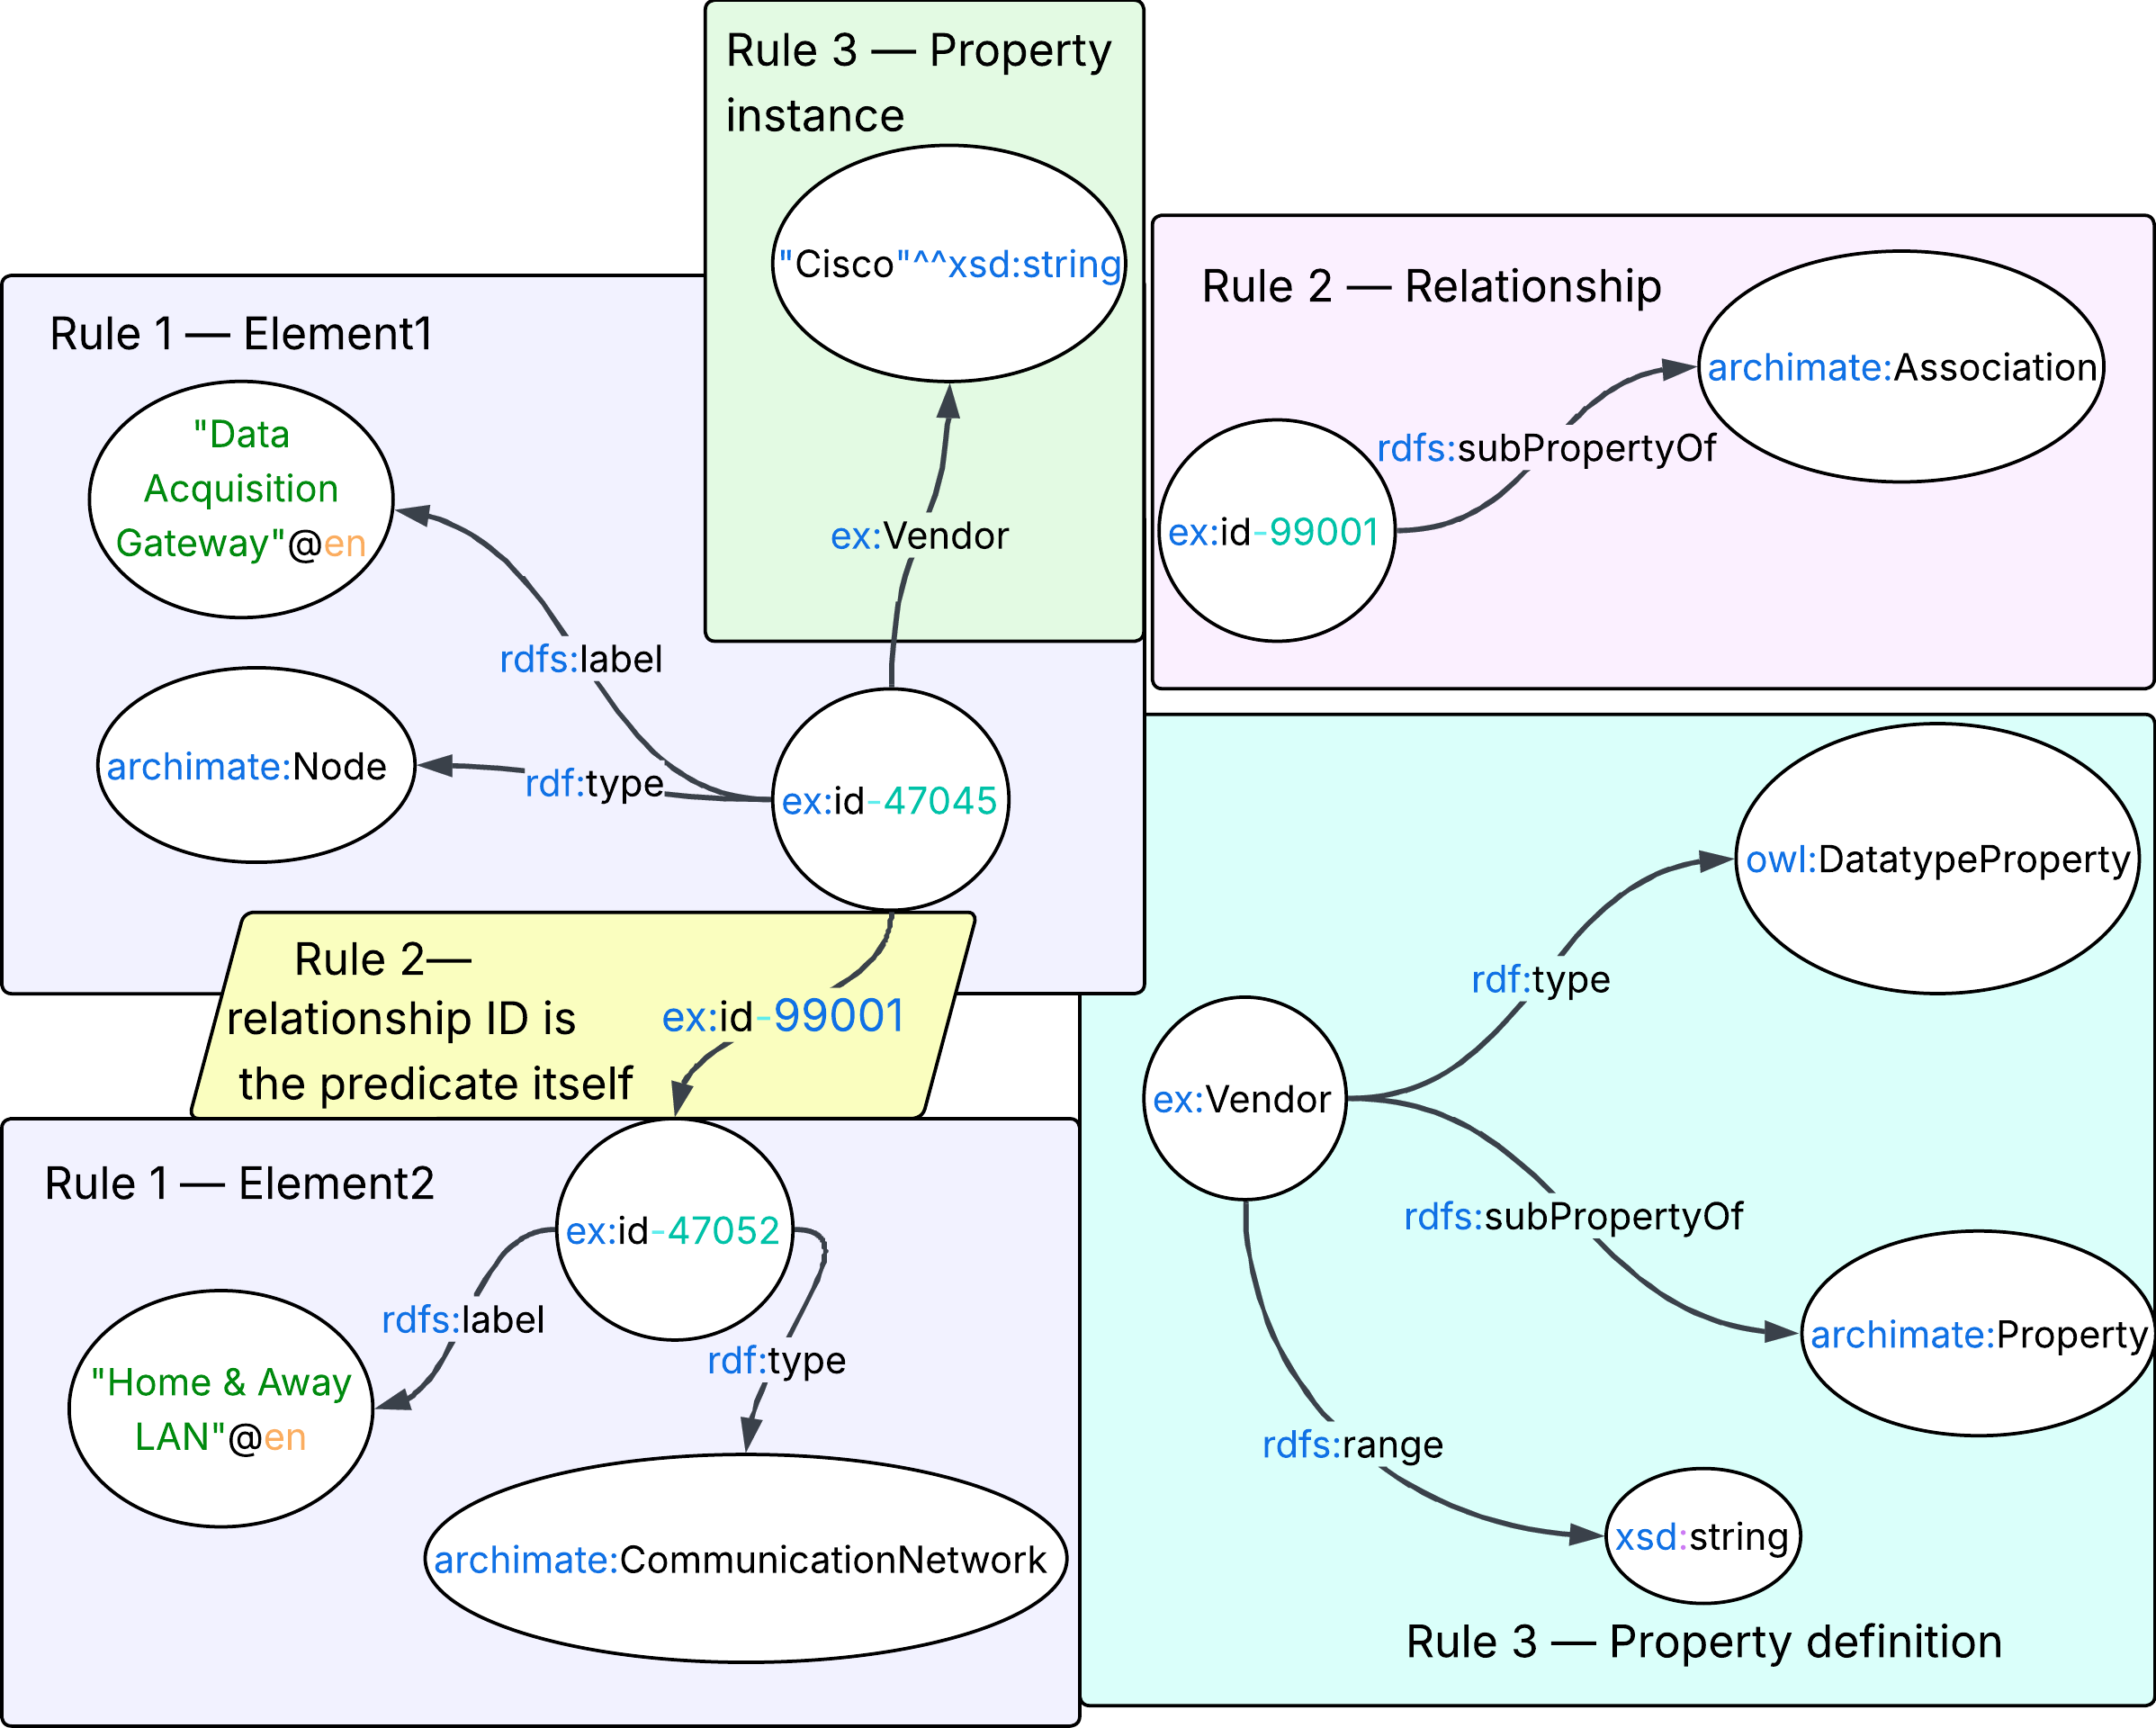
\includegraphics[width=\linewidth]{worked_example.png}
    \caption{EAKG representation of the input ArchiMate fragment in Listing~\ref{lst:worked-xml}}
    \label{fig:worked-rules}
\end{figure}
% ======================================================================
%  chapitre2.tex — Implementation
%  \input from main.tex — do not compile standalone.
% ======================================================================

\chapter{Implementation}
\label{chap:implementation}

This chapter describes the concrete implementation of the translation methodology presented in \autoref{chap:translation}. The translator (\texttt{archimate\_to\_eakg.py}) converts an ArchiMate Model Exchange File Format XML document into an RDF/OWL knowledge graph. Enrichment is performed directly in the triplestore (GraphDB) by loading the ontologies and inserting necessary triples using SPARQL queries. The entire stack is built on open standards and open-source tooling. A YARRRML implementation of the translation rules was provided as a contribution by Amel BELMAKSENE to the work.

% ------------------------------------------------------------------
\section{Architecture of the Translator}
\label{sec:translator}

\begin{figure}[H]
    \centering
    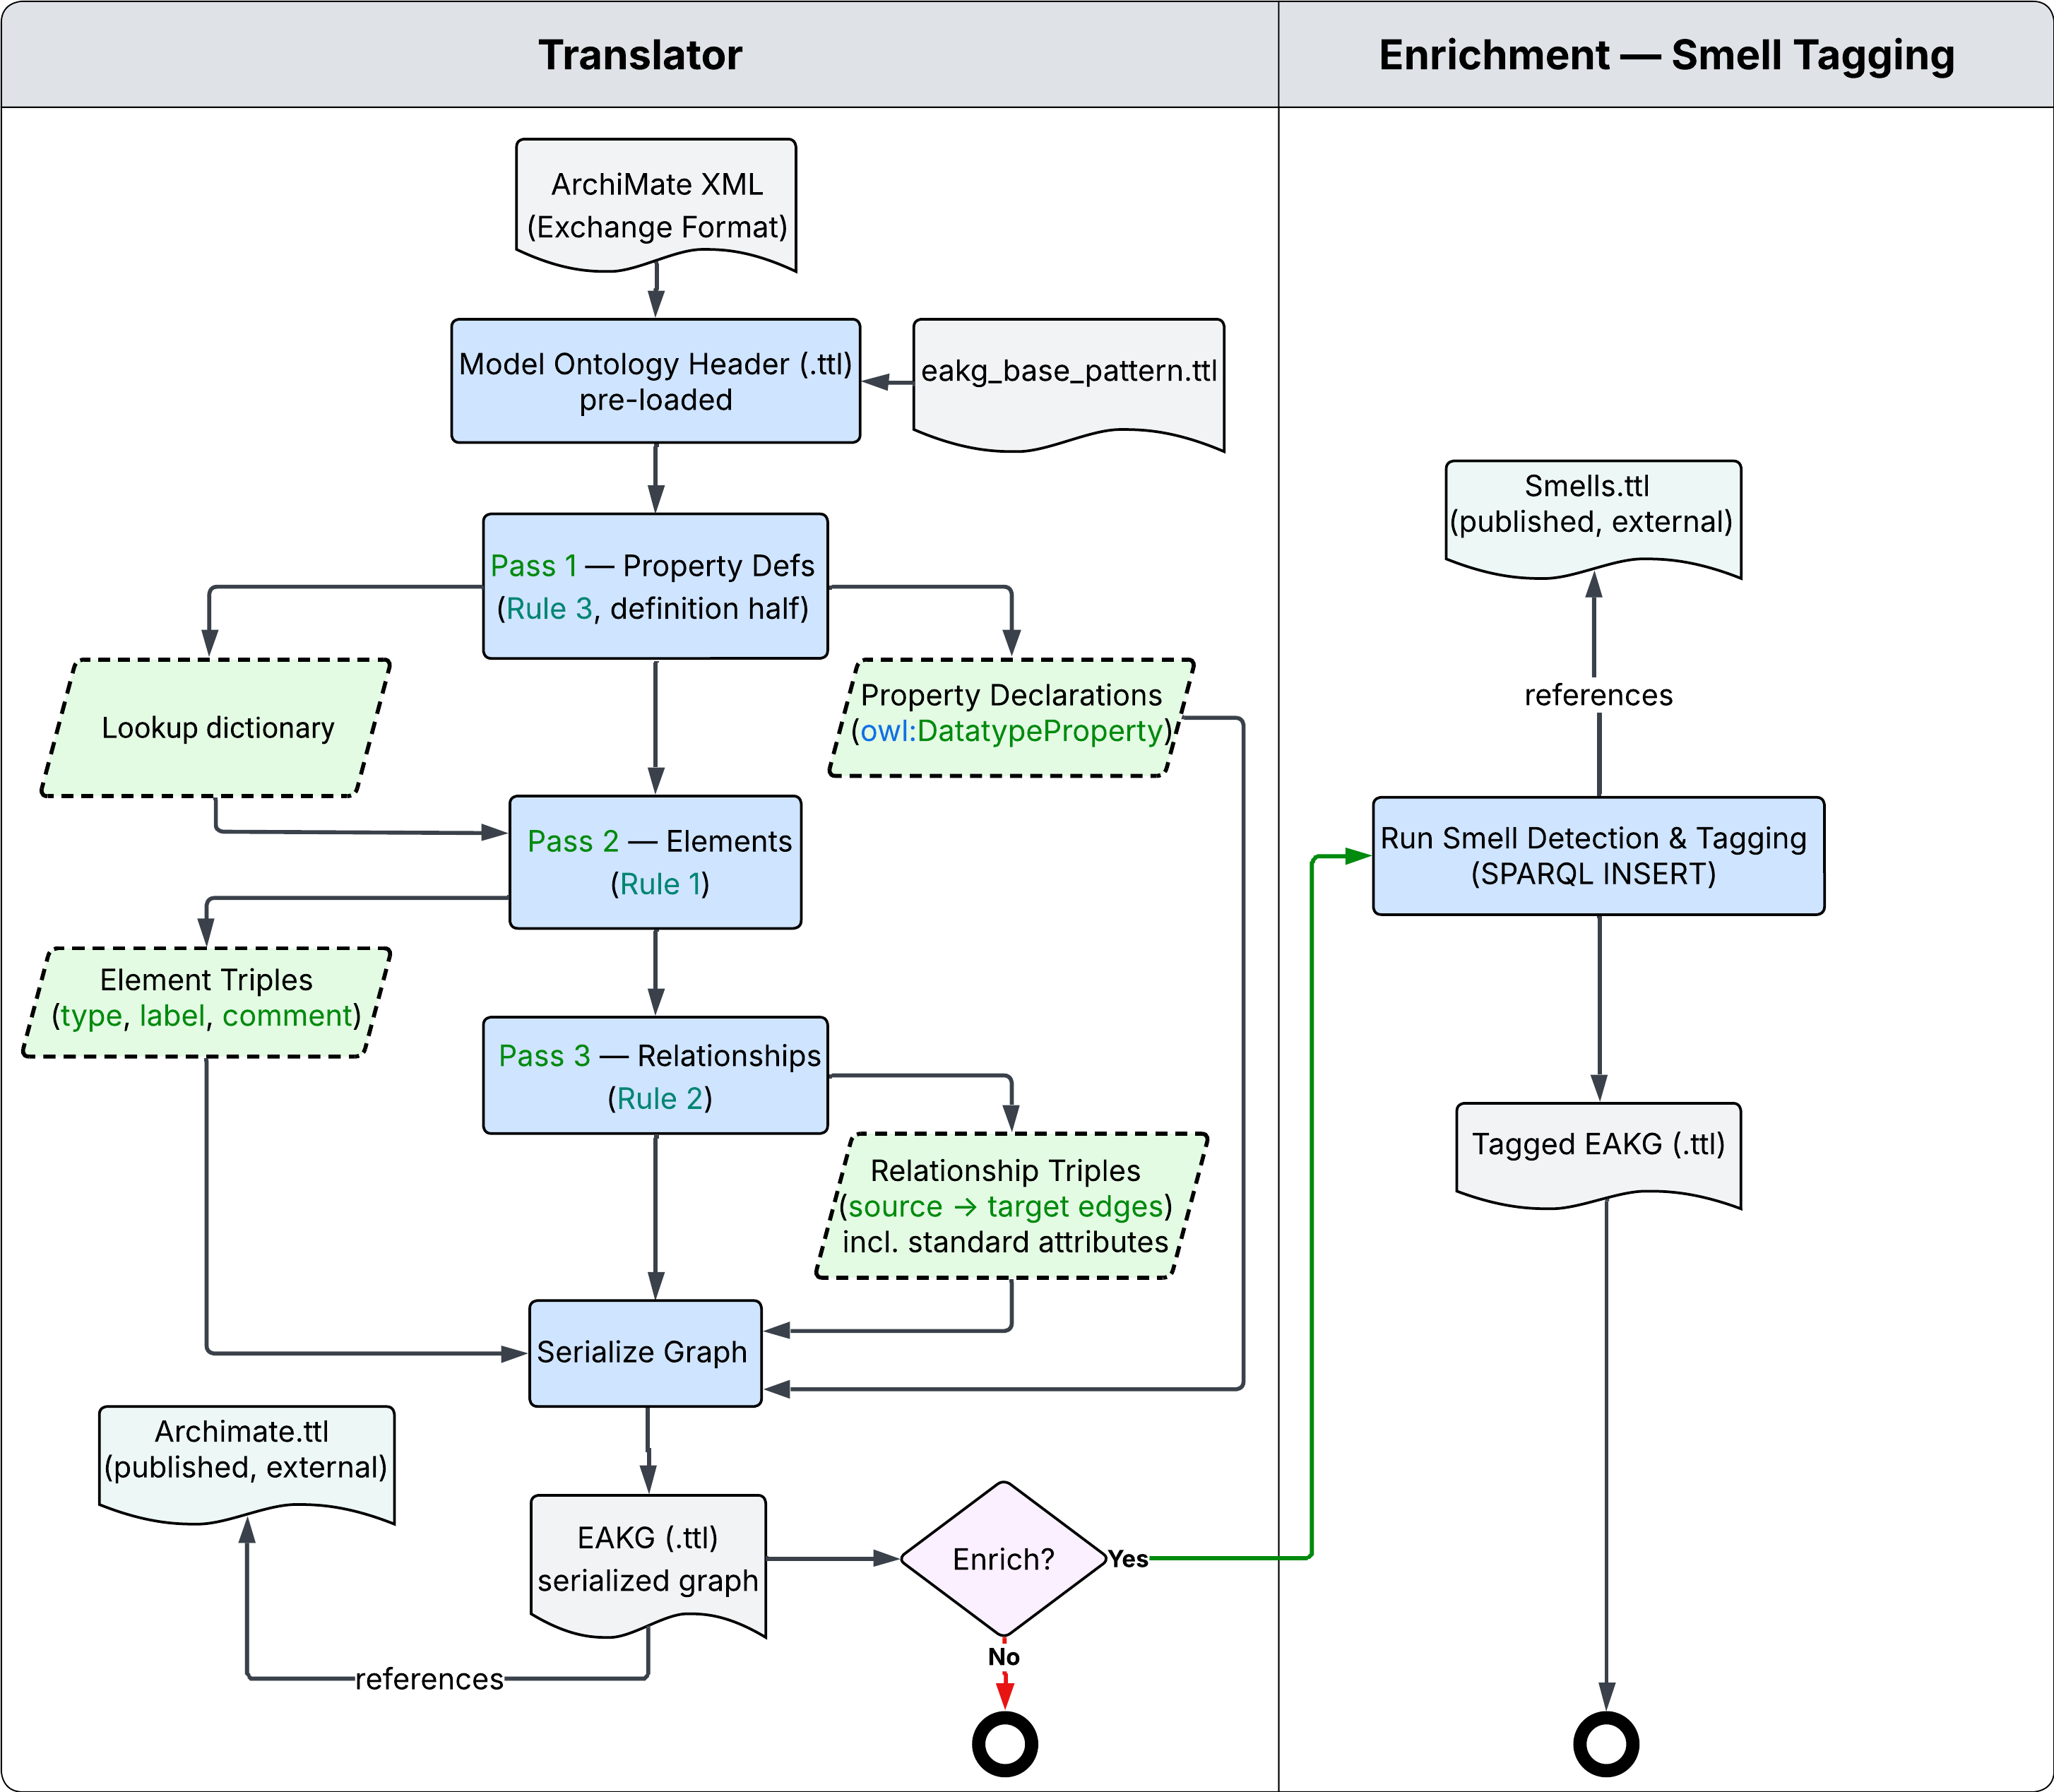
\includegraphics[width=\linewidth]{implementation_updated.png}
    \caption{Translator and enrichment pipeline}
    \label{fig:translator-enrichment}
\end{figure}

The translator (\texttt{archimate\_to\_eakg.py}) takes an ArchiMate Model Exchange File Format (v3.1) XML file as input and produces an Enterprise Architecture Knowledge Graph serialized as a Turtle\parencite{turtle} (\texttt{.ttl}) file. The program is invoked from the command line:

\begin{verbatim}
python archimate_to_eakg.py <input.xml> [output.ttl]
\end{verbatim}

If no output path is given, the result is written to \texttt{eakg\_output.ttl} in the same directory as the input file.

The translation pipeline is organized into three sequential passes over the XML document, each implementing one of the core translation rules defined in \autoref{chap:translation}.

% ------------------------------------------------------------------
\subsection{Namespaces and Lookup Tables}
\label{subsec:namespaces}

The program begins by declaring the RDF namespaces used throughout the graph. Three namespaces are central to the output:

\begin{itemize}
    \item \texttt{ex:} (\texttt{http://www.example.org/eakg\#}) --- used for all individual elements, relationships, and property predicates that originate from the concrete ArchiMate model.
    \item \texttt{archimate:} (\texttt{http://purl.org/eakg/archimate\#}) --- the ArchiMate metamodel vocabulary represented by the ontology described in \autoref{sec:ontology}, published at a persistent URL. Classes such as \texttt{archimate:BusinessActor}, relationship types such as \texttt{archimate:Association}, and schema-fixed attributes such as \texttt{archimate:accessType} are defined under this namespace.
    \item \texttt{smells:} (\texttt{http://purl.org/eakg/smells\#}) --- the EA smell ontology, also published at a persistent URL. Defines the \texttt{smells:hasSmell} predicate and seven smell individuals used during the enrichment phase.
\end{itemize}

A lookup table maps ArchiMate primitive type strings to their corresponding XSD datatype URIs. This table is used during Pass~1 to assign the correct \texttt{rdfs:range} to each property definition:

\begin{verbatim}
  "string"  -> xsd:string
  "boolean" -> xsd:boolean
  "integer" -> xsd:integer
  "float"   -> xsd:float
  "date"    -> xsd:date
  "time"    -> xsd:time
  "number"  -> xsd:decimal
\end{verbatim}

% ------------------------------------------------------------------
\subsection{Utility Functions}
\label{subsec:utilities}

Several helper functions are shared across passes:

\begin{itemize}
    \item \texttt{id\_to\_iri} and \texttt{property\_name\_to\_iri} create stable, sanitized IRIs; \texttt{resolve\_archimate\_class} maps XML types to ontology classes; and \texttt{emit\_lang\_literals} preserves language-tagged names and documentation. Detailed behavior is summarized in Annex~B.
\end{itemize}

% ------------------------------------------------------------------
\subsection{Pass 1: Property Definitions (Rule 3 --- Definition Half)}
\label{subsec:pass1}

The first pass registers property predicates and their XSD ranges, returning the lookup dictionary needed by the element and relationship passes.

% ------------------------------------------------------------------
\subsection{Pass 2: Elements (Rule 1)}
\label{subsec:pass2}

The second pass converts each XML element into a typed named individual, emits multilingual labels and comments, and writes its property values as direct triples using the Pass~1 dictionary.

% ------------------------------------------------------------------
\subsection{Pass 3: Relationships (Rule 2)}
\label{subsec:pass3}

The third pass turns each relationship identifier into an object-property predicate, links it to its ArchiMate relationship class, and emits the source-to-target triple plus any metadata and property values.

% ------------------------------------------------------------------
\subsection{Knowledge Graph Deployment and Usage}
\label{subsec:kg-deployment-usage}

The resulting KG then loaded in the triple store (importing the turtle file in GraphDB), and also import the Archimate Ontology which includes definition and hierarchy of used classes/predicate. Then the graph can be visualized or queried using SPARQL.

% ------------------------------------------------------------------
\section{Enrichment: Ontology Loading and Smell Tagging}
\label{sec:enrichment}

Enrichment is performed directly in the triplestore after loading the created graph.

\subsection{Ontology Loading}
\label{subsec:ontology-loading}

The enrichment ontology EA smell ontology in our case is loaded into the triplestore via its persistent URL \texttt{http://purl.org/eakg/smells}), alongside the translated model. This allow using resources and predicate defined in the enrichment ontology.

\subsection{EA Smell Tagging}
\label{subsec:smell-tagging}

Once the ontologies and model are loaded and RDFS reasoning is active, EA smells are detected and tagged using SPARQL queries. For each smell, the process follows two steps:

\begin{enumerate}
    \item A \textbf{detection \texttt{SELECT}} query identifies the affected elements or relations.
    \item A \textbf{tagging \texttt{INSERT}} query materializes a \texttt{smells:hasSmell} triple on each affected resource, using the same detection logic as its \texttt{WHERE} clause.
\end{enumerate}

The detection queries are unchanged from the analytical queries presented in Chapter~\ref{chap:queries}. The tagging queries are presented alongside them. Once tagged, affected resources can be retrieved with a single generic query by specifying the smell URI, and tags can be selectively reset.

% ------------------------------------------------------------------
\section{Tools and Technology Stack}
\label{sec:tools}

The implementation relies on the following tools and technologies:

\begin{itemize}
    \item \textbf{Python 3} as the programming language for both the translator and the enrichment module.
    \item \textbf{rdflib} (Python library) for constructing, manipulating, and serializing RDF graphs \parencite{rdflib2024}. It provides native support for Turtle, N-Triples, and other RDF serialization formats, as well as namespace management and literal typing.
    \item \textbf{xml.etree.ElementTree} (Python standard library) for parsing the ArchiMate Model Exchange File Format XML documents.
    \item \textbf{GraphDB} (Ontotext) as the target triplestore for deploying the resulting EAKG \parencite{ontotext2024graphdb}. GraphDB supports SPARQL 1.1 querying and RDFS reasoning, which enables the sub-property inference chains relied upon by our translation rules.
    \item \textbf{SPARQL 1.1} as the query language for analyzing the deployed knowledge graph.
    \item \textbf{RDFS reasoning} for inferring implicit relationships through the \texttt{rdfs:subPropertyOf} and \texttt{rdfs:subClassOf} hierarchies defined in the base ontology. This allows queries to match, for example, all \texttt{archimate:DependencyRelationship} instances without enumerating every concrete sub-property.
\end{itemize}

% ======================================================================
%  chapitre3.tex — SPARQL Querying and Analysis
%  \input from main.tex — do not compile standalone.
% ======================================================================

\chapter{SPARQL Querying and Analysis}
\label{chap:queries}

This chapter demonstrates how the EAKG, once deployed in a SPARQL-enabled triplestore such as GraphDB, can be queried and analyzed. We begin with simple exploratory queries, then present a gap analysis technique that leverages the knowledge graph to automate parts of the TOGAF ADM process, and finally describe a set of EA smell detection queries.

% ==================================================================
\section{Simple and Exploratory Queries}
\label{sec:simple-queries}

% ------------------------------------------------------------------
\subsection{Dependency Chain Queries}
\label{subsec:dependency-chains}

Dependency chain queries discover dependencies between elements. These dependencies can be direct or follow a transitive chain using the SPARQL property path operator (\texttt{+}). For example, the following query finds all elements that a given component (here, ``Document Management Back-Up Server'') depends on, traversing both \texttt{archimate:DependencyRelationship} and \texttt{archimate:StructuralRelationship} edges:

\begin{lstlisting}[caption={Dependency chain: elements that a given component depends on}]
PREFIX rdf:  <http://www.w3.org/1999/02/22-rdf-syntax-ns#>
PREFIX rdfs: <http://www.w3.org/2000/01/rdf-schema#>
PREFIX archimate: <http://purl.org/eakg/archimate#>
PREFIX smells: <http://purl.org/eakg/smells#>

SELECT DISTINCT ?component ?service ?serviceName
WHERE {
    ?component rdfs:label "Document Management Back-Up Server"@en .
    ?service (archimate:DependencyRelationship
             |archimate:StructuralRelationship)+ ?component .
    ?service rdf:type archimate:Element ;
             rdfs:label ?serviceName .
}
\end{lstlisting}

All subsequent queries in this chapter and in the Annex assume the same prefixes unless otherwise noted.

Dependency chains can also be traversed in the opposite direction. For example, the query below lists what depends on a given component (here, ``PaaS Services''):

\textit{(full query: see Annex, Listing A.1)}

\begin{table}[H]
\centering
\caption{Dependency chain results for ``Document Management Back-Up Server''}
\label{tab:dependency-results}
\small
\begin{tabularx}{\linewidth}{l l X}
\toprule
\textbf{component} & \textbf{service} & \textbf{service name} \\
\midrule
ex:id-47094 & ex:id-47052 & Home \& Away LAN \\
ex:id-47094 & ex:id-47506 & Homeowner's \& Travel Back Office \\
ex:id-47094 & ex:id-47045 & Data Acquisition Gateway \\
ex:id-47094 & ex:id-47088 & FO General-Purpose Server \\
ex:id-47094 & ex:id-47090 & FO Web Hosting Server \\
ex:id-47094 & ex:id-47508 & Home \& Away Headquarters \\
ex:id-47094 & ex:id-47100 & PaaS Services \\
ex:id-47094 & ex:id-47393 & Project: Data Warehousing and BI \\
ex:id-47094 & ex:id-47501 & Front Office \\
\bottomrule
\end{tabularx}
\end{table}

% ------------------------------------------------------------------
\subsection{Orphan Element Detection}
\label{subsec:orphan-elements}

A useful model quality check is to find elements that have no relationship with any other element---orphan nodes that may have been forgotten during modeling:

\begin{lstlisting}[caption={Detect orphan elements (no incoming or outgoing relationships)}]
SELECT ?element ?elementName
WHERE {
    ?element rdfs:label ?elementName ;
             a archimate:Element .
    FILTER NOT EXISTS {
        ?element archimate:Relationship ?target .
        ?target a archimate:Element .
    }
    FILTER NOT EXISTS {
        ?source archimate:Relationship ?element .
        ?source a archimate:Element .
    }
}
\end{lstlisting}

The query returns 15 orphan elements in the ArchiSurance model, including Product Information, Insurance, Insurance Policy, Commission, Bank, Business Intelligence Team, and several customer-channel elements.

% ------------------------------------------------------------------
\subsection{Most Connected Elements}
\label{subsec:most-connected}

Sorting elements by their total number of relationships (incoming and outgoing) helps identify the most central components of the architecture:

\begin{lstlisting}[caption={Rank elements by total number of relationships}]
SELECT ?element ?elementName
       ((COALESCE(?in,0) + COALESCE(?out,0)) AS ?relations)
WHERE {
    ?element rdfs:label ?elementName .
    ?element a archimate:Element .
    OPTIONAL {
        SELECT ?element (COUNT(DISTINCT ?s) AS ?in)
        WHERE {
            ?s ?rel ?element .
            ?rel rdfs:subPropertyOf* archimate:Relationship .
        }
        GROUP BY ?element
    }
    OPTIONAL {
        SELECT ?element (COUNT(DISTINCT ?t) AS ?out)
        WHERE {
            ?element ?rel ?t .
            ?rel rdfs:subPropertyOf* archimate:Relationship .
        }
        GROUP BY ?element
    }
}
ORDER BY DESC(?relations)
\end{lstlisting}

\begin{table}[H]
\centering
\caption{Eight most connected elements}
\label{tab:most-connected-results}
\small
\begin{tabularx}{\linewidth}{l X r}
\toprule
\textbf{element} & \textbf{element name} & \textbf{relations} \\
\midrule
ex:id-46339 & Target: CRM, Back Office and Data Warehouse Operational & 36 \\
ex:id-46304 & ArchiSurance Back Office Suite & 23 \\
ex:id-47396 & Baseline & 23 \\
ex:id-46637 & Finance & 18 \\
ex:id-46860 & Document Management System & 16 \\
ex:id-46330 & Manage Policies and Claims & 15 \\
ex:id-46918 & Home \& Away Policy Administration & 15 \\
ex:id-46369 & Serve Customers & 14 \\
\bottomrule
\end{tabularx}
\end{table}

% ------------------------------------------------------------------
\subsection{Layer Listings}
\label{subsec:layer-listings}

The following query lists all elements together with their ArchiMate layer classification, exploiting the ontology's class hierarchy:

\textit{(full query: see Annex, Listing A.2)}

Elements can also be listed by the relationships between layers. The cross-layer count below reports the four Application-to-Business type pairs returned by the query.

\textit{(full query: see Annex, Listing A.3)}

\begin{table}[H]
\centering
\caption{Relationships from Application Layer to Business Layer}
\label{tab:cross-layer-results}
\small
\begin{tabularx}{\linewidth}{X X r}
\toprule
\textbf{source type} & \textbf{target type} & \textbf{count} \\
\midrule
archimate:ApplicationComponent & archimate:BusinessFunction & 22 \\
archimate:ApplicationService & archimate:BusinessProcess & 16 \\
archimate:DataObject & archimate:BusinessObject & 3 \\
archimate:ApplicationProcess & archimate:BusinessProcess & 1 \\
\bottomrule
\end{tabularx}
\end{table}

% ==================================================================
\section{Gap Analysis}
\label{sec:gap-analysis}

\subsection{The TOGAF Gap Analysis Technique}
\label{subsec:togaf-gap}

According to the \textit{TOGAF}\textsuperscript{\textregistered} Standard---ADM Technique, Gap Analysis is a technique used to validate an architecture that is being developed \parencite{opengroup2022togaf}. The basic premise is to highlight a shortfall between the Baseline Architecture and the Target Architecture; that is, items that have been deliberately omitted, accidentally left out, or not yet defined.

In other words, Gap Analysis is the process of comparing the current architecture baseline with the new architecture we want to achieve in the future (target) to identify what needs to be added, removed, or modified. A key step in validating the architecture is to identify what has been forgotten.

\noindent\textbf{Suggested Method by the Standard}\par

The standard suggests the following matrix-based method:

\begin{itemize}
    \item Draw a matrix where the Architecture Building Blocks (ABBs) from the baseline architecture are listed per rows, and ABBs present in the target architecture are listed per columns.
    \item Add a last row labeled ``New'' and a last column labeled ``Eliminated.''
    \item ABBs available in both architectures are marked with ``Included'' at the intersecting cell.
    \item ABBs that appear only in the baseline architecture should be reviewed to determine if they were correctly removed or forgotten. If correctly eliminated, mark them in the appropriate ``Eliminated'' cell; otherwise they must be readdressed in the next iteration.
    \item ABBs that appear only in the target architecture are marked in the intersecting cell with the ``New'' row as a gap.
\end{itemize}

When the matrix is completed, ``Eliminated'' and ``New'' marks represent gaps that should be explained---either as correctly eliminated items or as items that need to be addressed by reinstating or developing/procuring the new building block.

% ------------------------------------------------------------------
\subsection{ArchiMate Representation}
\label{subsec:archimate-gap}

In ArchiMate, the ``Implementation and Migration Layer'' includes elements that model the evolution of enterprise architecture through programs and projects \parencite{opengroup2023archimate}. The relevant element types are:

\begin{enumerate}
    \item \textbf{Work Package}: a series of actions identified and designated to achieve specific results within specified time and resource constraints. It has a start and end, and produces goals, outcomes, or deliverables.
    \item \textbf{Deliverable}: represents a result of a Work Package---reports, papers, services, software, physical products, etc.
    \item \textbf{Plateau}: represents a relatively stable state of the architecture that exists during a limited period of time. Plateaus show the enterprise at incremental states reflecting periods of transition between the Baseline and Target Architectures, and allow grouping work packages into portfolios and programs.
    \item \textbf{Gap}: represents a statement of difference between two plateaus. It is associated with two plateaus and represents the difference between them.
\end{enumerate}

% ------------------------------------------------------------------
\subsection{Knowledge Graph Role in Gap Analysis}
\label{subsec:kg-gap}

By transforming the ArchiMate model into a knowledge graph, we can automate the creation of the matrix in the Gap Analysis process. By querying the Knowledge Graph we can extract the list of ``Kept,'' ``Eliminated,'' and ``New'' ABBs. After evaluation by the architect, those elements are marked by linking them to the ``Gap'' node with the appropriate property, to keep track of taken decisions in the knowledge graph.

\noindent\textbf{Queries to List Gap Elements}\par

Three queries extract the gap classification directly from the knowledge graph:

\begin{enumerate}
    \item \textbf{ABBs present in both architectures (Kept).} This query returns the elements aggregated by both the baseline and target plateaus. \textit{(full query: see Annex, Listing A.4)}
    \item \textbf{ABBs present only in the baseline (candidates for elimination).} This query identifies elements that belong to the baseline plateau but are absent from the target plateau. \textit{(full query: see Annex, Listing A.5)}
    \item \textbf{ABBs present only in the target (new gaps).} This query identifies elements introduced in the target plateau that do not exist in the baseline plateau. \textit{(full query: see Annex, Listing A.6)}
\end{enumerate}

\noindent\textbf{Marking Elements After Review}\par

We use project-specific RDF properties to link the ``Gap'' node with each element that presents a gap, which allows us to mark elements with the appropriate decision after review:

\begin{itemize}
    \item \texttt{ex:gapNew} for new ABBs to be produced/procured.
    \item \texttt{ex:gapInclude} for ABBs to be kept, which has a sub-property \texttt{ex:gapImproved} for kept ABBs that require improvement.
    \item \texttt{ex:gapEliminated} for ABBs correctly removed from the architecture.
\end{itemize}

% ------------------------------------------------------------------
\subsection{Example: ArchiSurance Case Study}
\label{subsec:gap-example}

Using the ArchiSurance case study \parencite{jonkers2016archisurance}, we can model the evolution with a ``Gap'' between two plateaus:

\begin{itemize}
    \item The \textbf{baseline plateau} aggregates: Web Portal, Call Center Application, Legal Expense CRM System, General CRM System, Home \& Away Financial Application, Home \& Away Policy Administration, Auto Insurance Application, Legal Expense Back-Office System, Document Management System.
    \item The \textbf{target plateau} aggregates: Web Portal, Call Center Application, General CRM System, Document Management System, ArchiSurance Back-Office Suite, Data Warehousing Solution, MyArchiSurance Mobile App.
\end{itemize}

In the knowledge graph, each plateau is represented with a node that has an ``aggregate'' property linking it to all its included elements, and a ``Gap'' node is associated with both plateau nodes. Using the previous queries, we can list the gap classification without the need to draw the matrix:

\begin{itemize}
    \item \textbf{Kept}: Web Portal, Call Center Application, General CRM System, Document Management System.
    \item \textbf{Eliminated}: Legal Expense CRM System, Home \& Away Financial Application, Home \& Away Policy Administration, Auto Insurance Application, Legal Expense Back-Office System.
    \item \textbf{New}: ArchiSurance Back-Office Suite, Data Warehousing Solution, MyArchiSurance Mobile App.
\end{itemize}

The following combined query classifies elements from the gap analysis according to the TOGAF gap analysis matrix, using concrete identifiers from the ArchiSurance model:

\begin{lstlisting}[caption={Classify elements as Kept, Eliminated, or New in one query}]
# Newly introduced prefix for this query.
PREFIX ex: <http://www.example.org/eakg#>

SELECT ?ABB ?label ?state
WHERE {
    BIND(ex:id-46339 AS ?target)
    BIND(ex:id-47396 AS ?baseline)
    {
        ?baseline archimate:Aggregation ?ABB .
        ?target archimate:Aggregation ?ABB .
        ?ABB rdfs:label ?label .
        BIND("Kept" AS ?state)
    }
    UNION
    {
        ?baseline archimate:Aggregation ?ABB .
        FILTER NOT EXISTS {
            ?target archimate:Aggregation ?ABB .
        }
        ?ABB rdfs:label ?label .
        BIND("Eliminated" AS ?state)
    }
    UNION
    {
        ?target archimate:Aggregation ?ABB .
        FILTER NOT EXISTS {
            ?baseline archimate:Aggregation ?ABB .
        }
        ?ABB rdfs:label ?label .
        BIND("New" AS ?state)
    }
}
\end{lstlisting}

After reviewing each element, we mark it with the appropriate property by inserting triples with the ``Gap'' node. The following SPARQL Update query shows how decisions are recorded:

\textit{(full query: see Annex, Listing A.7)}

% ------------------------------------------------------------------
\subsection{Further Exploration: Ontology-Based EA Evolution}
\label{subsec:gap-further}

A small ontology to model enterprise evolution is proposed in \parencite{silva2017evolution}, taking advantage of computer agents to aid communication and analysis of EA model evolution. The key concepts of this ontology are:

\begin{itemize}
    \item An \textbf{IT Project} acts as an enabler of EA evolution by applying a set of \textbf{Transformations}.
    \item A Transformation can be decomposed into smaller \textbf{Changes}, each altering the life-cycle of an EA Description (element or relationship).
    \item To keep track of motivation and interested parties, the ontology introduces \textbf{Stakeholder} (who has one or more drivers) and \textbf{Driver} (an internal or external motivation/condition that makes the change necessary).
    \item This model keeps information about how the EA was changed, when those changes happened, who involved those changes, and why.
\end{itemize}

The authors proposed a set of Description Logic (DL) queries to answer questions that help decision-making and facilitate change analysis. In our case, DL queries can be replaced with equivalent SPARQL queries into the knowledge graph.

\begin{samepage}
For example, to find what transformations are applied by an IT project named ``Back-Office System Integration,'' the proposed DL query:

\begin{lstlisting}[language=, basicstyle=\small\ttfamily, frame=single]
Transformation and
  applied_by some
    (IT_Project and
     hasName value "Back-Office_System_Integration")
\end{lstlisting}
\end{samepage}

can be expressed as the following SPARQL equivalent:

\textit{(full query: see Annex, Listing A.8)}

% ==================================================================
\section{EA Smells Detection Queries}
\label{sec:smells}

Enterprise Architecture Smells are recurring patterns in an EA model that indicate potential design problems \parencite{salentin2020smells}. The following subsections present SPARQL queries that detect and tag several categories of smells, leveraging the RDFS reasoning capabilities of the triplestore. For each smell, a detection \texttt{SELECT} identifies the affected resources and a tagging \texttt{INSERT} materializes a \texttt{smells:hasSmell} triple on each one. These queries were tested on the demonstration model from \parencite{salentin2020smells}, which was designed to exhibit each smell.

% ------------------------------------------------------------------
\subsection{Structural and Connectivity Smells}
\label{subsec:structural-smells}

\noindent\textbf{Cyclic Dependency}\par

\textbf{The Concept:} Elements should not be stuck in an endless loop of depending on one another. This behavior is illustrated in the demonstration model of \parencite{salentin2020smells}.

\textbf{The Detection Logic:} We target the \texttt{archimate:DependencyRelationship} hierarchy and scan the graph globally to match unbroken chains of these dependency edges. If traversing that chain eventually leads right back to the exact same starting node, a cycle is detected.

\textit{(full query: see Annex, Listing A.9)}

Each element in the cycle is tagged with \texttt{smells:CyclicDependency}. \textit{(tagging query: see Annex, Listing A.14)}

\noindent\textbf{Shared Persistency}\par

\textbf{The Concept:} Higher-level business components should not bypass the application layer to talk directly to the same backend database. This behavior is illustrated in the demonstration model of \parencite{salentin2020smells}, where it is treated together with Strict Layers Violation rather than as a separately defined smell.

\textbf{The Detection Logic:} We isolate \texttt{archimate:PassiveStructureElement} nodes, which represent data. We then look for instances where two or more distinct elements from the \texttt{archimate:BusinessLayer} have an \texttt{archimate:Access} edge pointing directly to that exact same data node.

\textit{(full query: see Annex, Listing A.10)}

The shared data node is tagged with \texttt{smells:SharedPersistency}. \textit{(tagging query: see Annex, Listing A.15)}

\noindent\textbf{Strict Layers Violation}\par

\textbf{The Concept:} The architecture should follow a strict top-down hierarchy (Business $\rightarrow$ Application $\rightarrow$ Technology). Skipping an intermediate layer by establishing a direct link between the Business layer and the Technology layer breaks this core design principle. As a best practice, no direct architectural relationships of any kind or direction should bridge these layers directly without traversing the application layer.

\textbf{The Detection Logic:} We search for any direct relationship where one connected node belongs to the \texttt{archimate:BusinessLayer} and the other belongs to the \texttt{archimate:TechnologyLayer}. By checking both directions, we confirm that the \texttt{archimate:ApplicationLayer} has been entirely bypassed, regardless of how the relationship was originally oriented in the model.

\begin{lstlisting}[caption={Detect strict layers violation}]
SELECT DISTINCT ?nodeA ?nodeB ?relation ?direction
WHERE {
    {
        ?nodeA a archimate:BusinessLayer .
        ?nodeB a archimate:TechnologyLayer .
        ?nodeA ?relation ?nodeB .
        BIND("Business_to_Tech" AS ?direction)
    }
    UNION
    {
        ?nodeA a archimate:TechnologyLayer .
        ?nodeB a archimate:BusinessLayer .
        ?nodeA ?relation ?nodeB .
        BIND("Tech_to_Business" AS ?direction)
    }
    ?relation rdfs:subPropertyOf* archimate:Relationship .
    FILTER(STRSTARTS(STR(?relation),
           "http://www.example.org/eakg#id"))
}
\end{lstlisting}

The offending relationship edge is tagged with \texttt{smells:StrictLayersViolation}. \textit{(tagging query: see Annex, Listing A.16)}

% ------------------------------------------------------------------
\subsection{Service and Interaction Smells}
\label{subsec:service-smells}

\noindent\textbf{Chatty Service}\par

\textbf{The Concept:} A service should not be overly communicative, firing off a massive number of granular requests to a vast array of other services. \parencite{salentin2020smells} state that a service related to a high number of other services may indicate this smell.

\textbf{The Detection Logic:} We target service nodes (\texttt{archimate:ApplicationService}, \texttt{archimate:BusinessService}) and count the total number of unique elements they connect to. If that count exceeds a defined acceptable threshold, the service is flagged.

\begin{lstlisting}[caption={Detect chatty services (threshold: 10 connections)}]
SELECT ?service ?label
       (COUNT(DISTINCT ?connectedElement) AS ?connectionCount)
WHERE {
    ?service a ?serviceType .
    FILTER (?serviceType IN (archimate:ApplicationService,
                             archimate:BusinessService))
    ?service rdfs:label ?label .
    {
        ?service ?relation ?connectedElement .
    }
    UNION
    {
        ?connectedElement ?relation ?service .
    }
    ?relation rdfs:subPropertyOf* archimate:Relationship .
    FILTER(STRSTARTS(STR(?relation),
           "http://www.example.org/eakg#id"))
}
GROUP BY ?service ?label
HAVING (COUNT(DISTINCT ?connectedElement) >= 10)
\end{lstlisting}

The overly communicative service node is tagged with \texttt{smells:ChattyService}. \textit{(tagging query: see Annex, Listing A.17)}

\noindent\textbf{Data Service}\par

\textbf{The Concept:} A service should execute logic. If it only touches data objects and nothing else, it is just a weak data-access point. This smell is described in \parencite{salentin2020smells} as a service that only references data objects without relating to other components.

\textbf{The Detection Logic:} We isolate service nodes and evaluate their \emph{outgoing} relationships (where the service acts as the source). We identify services that have outgoing edges pointing to \texttt{archimate:PassiveStructureElement} nodes, but apply a strict filter to ensure they have \emph{zero} outgoing edges pointing to any \texttt{archimate:ActiveStructureElement} or \texttt{archimate:BehaviorElement}. Incoming edges (other components calling the service) are expected and are ignored by this filter.

\textit{(full query: see Annex, Listing A.11)}

The data-only service node is tagged with \texttt{smells:DataService}. \textit{(tagging query: see Annex, Listing A.18)}

% ------------------------------------------------------------------
\subsection{Model Quality Smells}
\label{subsec:quality-smells}

\noindent\textbf{Duplication}\par

\textbf{The Concept:} The model should not contain multiple distinct elements that share the exact same name. Sharing a name alone is treated as a smell, regardless of the elements' specific types. A similar case is illustrated in the demonstration model of \parencite{salentin2020smells}, based on name similarity rather than exact matching.

\textbf{The Detection Logic:} We compare the \texttt{rdfs:label} (the name) across the graph. If we find two or more distinct nodes (different IRIs) sharing the exact same label, they are flagged as duplicates.

\textit{(full query: see Annex, Listing A.12)}

Each element sharing its label with at least one other element is tagged with \texttt{smells:Duplication}. \textit{(tagging query: see Annex, Listing A.19)}

\noindent\textbf{Unnecessary Documentation}\par

\textbf{The Concept:} Model documentation should be concise. Huge walls of text clutter the repository. This smell is illustrated in the demonstration model of \parencite{salentin2020smells}, but no general threshold is stated.

\textbf{The Detection Logic:} We extract the \texttt{rdfs:comment} string literal for every element in the graph, calculate the character length of that string, and flag comments that exceed a specific character limit (e.g., 400 characters).

\textit{(full query: see Annex, Listing A.13)}

Any model resource exceeding the character limit is tagged with \texttt{smells:UnnecessaryDocumentation}. \textit{(tagging query: see Annex, Listing A.20)}

\subsection{Utility Functions}
\label{subsec:utility-functions}

The following query lists the elements tagged with a selected smell; replace
\texttt{smells:CyclicDependency} with any smell URI as needed:

\begin{lstlisting}[caption={View tagged elements for a specific smell}]
SELECT ?element ?label WHERE {
    ?element smells:hasSmell smells:CyclicDependency .
    OPTIONAL { ?element rdfs:label ?label . }
}
\end{lstlisting}

A corresponding query for resetting a selected smell tag is provided in Annex,
Listing A.21.

% ======================================================================
% chapitre4.tex - LLM-based natural-language evaluation
% \input from main.tex - do not compile standalone.
% ======================================================================

\chapter{Natural-Language Access to the Enterprise Architecture Knowledge Graph}
\label{chap:ai-evaluation}

\section{Objective and Motivation}
\label{sec:ai-objective}

The third objective of this work is to evaluate whether Enterprise Architecture models can be effectively explored and queried through natural-language interaction with a Large Language Model (LLM), and to what extent the representation format of the model---raw, translated, or made queryable---affects the quality of the answers produced.

While the previous objectives focused on defining a translation methodology from ArchiMate models to a Semantic Web ontology (RDF/OWL) and enriching the resulting Enterprise Architecture Knowledge Graph (EAKG) with structural and domain-specific knowledge such as EA smells, this objective addresses a practical question: does this translation effort improve an LLM's ability to reason about an EA model compared with simply providing the model in its native exchange format? Furthermore, does giving the LLM active access to the graph, rather than a static dump of it, change its performance?

To answer this, four experimental conditions were designed by varying two independent dimensions:
\begin{itemize}
    \item \textbf{Representation}: the raw ArchiMate Exchange Format model versus the translated EAKG ontology.
    \item \textbf{Access mode}: the full model provided statically as context versus the model made available as a live, queryable resource through a tool.
\end{itemize}

This comparison isolates the respective contributions of the translation methodology and interactive graph access rather than conflating the two.

\section{Test Setup}
\label{sec:ai-setup}

The four conditions were as follows:
\begin{enumerate}
    \item \textbf{Raw XML (static context).} The ArchiMate Exchange Format model, exported directly from the modeling tool, was provided in full as context. No translation or ontology mapping was applied.
    \item \textbf{Raw JSON (static context).} The same exchange-format model, converted to an equivalent JSON representation, was provided in full. This condition isolates XML versus JSON serialization while keeping the underlying information identical.
    \item \textbf{Translated EAKG ontology (static context).} The model was passed through the translation pipeline defined in this work, producing the EAKG in RDF/OWL. The resulting Turtle graph was provided as static context together with a general explanation of its namespaces, element and relationship mapping, property mapping, and layer and category resolution. No ArchiSurance-specific information was included in that explanation.
    \item \textbf{GraphDB live access (interactive).} The translated EAKG was loaded into GraphDB. The LLM received a SPARQL-query tool and the same schema explanation as in Test 3, and had to retrieve the information needed for each answer.
\end{enumerate}

Figure~\ref{fig:tests-setup} summarizes the four experimental conditions and the distinction between static context and interactive graph access.

\begin{figure}[H]
    \centering
    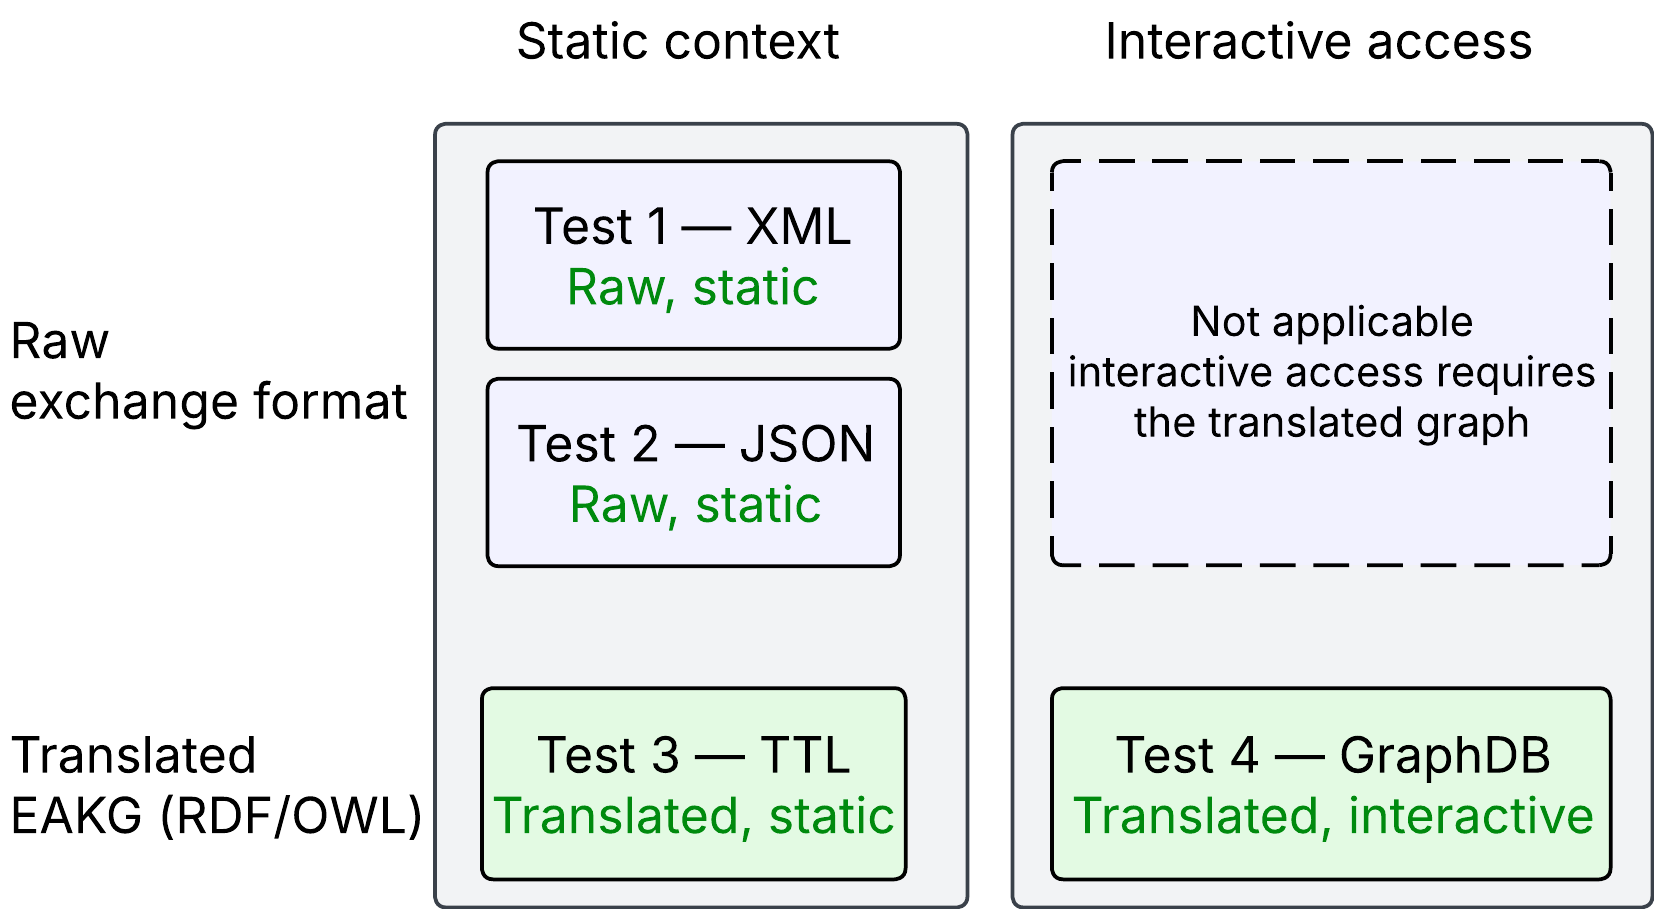
\includegraphics[width=\linewidth]{tests_setup.png}
    \caption{Experimental setup for the four LLM evaluation conditions}
    \label{fig:tests-setup}
\end{figure}

\section{Evaluation Methodology}
\label{sec:ai-methodology}

Answers produced under each condition were scored using a dedicated LLM-based grading procedure applied uniformly across all four tests.

\subsection{Ground Truth}
\label{subsec:ai-ground-truth}

The original ArchiSurance model in its native exchange format served as the sole authority for element identity, type, layer, and relationship existence, type, and direction. The accompanying Open Group ArchiSurance documentation was used only to resolve ambiguity and clarify intended semantics, never as a source of exact identifiers.

Although the grader was also an LLM, its role differed from that of the models under evaluation. The generation LLM in each test performed open-ended interpretation of a model it had to understand and reason about. The grading LLM was given the complete ground-truth model and performed a comparison task: it checked whether the elements, relationships, and directions cited in an answer matched what the ground truth explicitly contained. It was therefore verifying specific claims rather than independently reconstructing architectural knowledge.

\subsection{Grading Dimensions and Procedure}
\label{subsec:ai-grading}

Each answer was scored independently along three axes:
\begin{itemize}
    \item \textbf{Correctness} (0.00--1.00): how completely and accurately the answer matched what the ground truth supported, including penalties for missing elements, wrong relationship directions, and vague answers.
    \item \textbf{Grounding} (0.00--1.00): whether every substantive claim was traceable to a specific element or relationship identifier in the model.
    \item \textbf{Hallucination} (true/false): whether the answer contained an invented element, relationship, identifier, or type not present in the ground truth.
\end{itemize}

The final score was derived as a weighted combination of Correctness and Grounding using weights of 0.7 and 0.3. When hallucination was detected, the result was capped at 0.25. A correct refusal was scored 1.0 directly because it contained no specific claim to ground; if it also involved a hallucination, the same 0.25 cap applied.

For each question, the grader first determined the correct answer from the ground-truth model, then compared the generated answer with that reference. Special handling covered correct refusals, partial or missing identifiers, directional errors, and, for the interactive condition, answers that described a query strategy without reporting the instance-level results retrieved from the graph. Failed runs caused by tool or API errors were excluded from scoring and logged separately rather than penalized as incorrect answers.

The grading prompts for Tests 1--3 and Test 4 shared the same rubric, dimensions, score formula, and core edge-case rules. The Test 4 version additionally specified how to handle tool or API failures and query-strategy descriptions, which do not arise in the static-context conditions.

While the scoring was automated, targeted manual validation was performed on edge cases and ambiguous responses to ensure the integrity of the final scores.

\section{Results}
\label{sec:ai-results}

Each test was run twice on the same 26 questions. Answers were scored from 0 to 1, with correctness and grounding graded separately and hallucination flags recorded for each answer. Table~\ref{tab:ai-summary} summarizes the results; the complete question-level grid is provided in Annex~C.

\begin{table}[H]
\centering
\caption{Summary of the LLM evaluation results}
\label{tab:ai-summary}
\small
\resizebox{\linewidth}{!}{%
\begin{tabular}{l c c c c c c}
\toprule
\textbf{Test} & \textbf{Run 1} & \textbf{Run 2} & \textbf{Mean final score} & \textbf{Mean correctness} & \textbf{Mean grounding} & \textbf{Hallucinations} \\
\midrule
1 XML (static) & 0.70 & 0.90 & 0.80 & 0.83 & 0.86 & 7/52 (13\%) \\
2 JSON (static) & 0.74 & 0.88 & 0.81 & 0.81 & 0.91 & 4/52 (8\%) \\
3 TTL (static) & 0.58 & 0.75 & 0.67 & 0.72 & 0.82 & 12/52 (23\%) \\
4 GraphDB & 0.89 & 0.91 & 0.90 & 0.95 & 0.73 & 1/51 (2\%) \\
\bottomrule
\end{tabular}
}
\end{table}

Test 4 has 51 scored answers because one answer in Run 1 failed with a 503 error and was excluded. GraphDB access obtained the highest score and was the most stable across runs. The static Turtle dump obtained the lowest score, while XML and JSON were close to each other between the two extremes.

\section{Synthesis and Limitations}
\label{sec:ai-synthesis}

\subsection{Main Findings}
\label{subsec:ai-findings}

\textbf{Access mode mattered more than format.} Tests 3 and 4 used the same graph and schema explanation, yet GraphDB scored about 0.23 higher (0.67 versus 0.90) and produced no zero-score answers. The ontology was more useful when queried than when read as a static text dump.

\textbf{XML and JSON performed similarly.} Their mean scores were close (0.80 versus 0.81). JSON had better grounding (0.91 versus 0.86) and fewer hallucination flags (4 versus 7 of 52), whereas XML had slightly higher correctness (0.83 versus 0.81). With only two runs per condition, these differences indicate at most a mild advantage for JSON.

\textbf{Static conditions were less stable.} Run 2 exceeded Run 1 by 0.20 for XML, 0.14 for JSON, and 0.17 for TTL, whereas GraphDB changed by only 0.02. This pattern is suggestive but not conclusive.

\textbf{Failure modes differed by condition.} XML and JSON produced wrong relationship targets, wrong element types, and refusals for information present in the model. TTL mainly produced relation errors, including reversed directions and invented paths, as well as corrupted identifiers. GraphDB produced almost no direction or identifier errors; its only hallucination was a relation between real elements that was not present in the graph.

\textbf{Correctness and grounding should be read separately.} GraphDB had the highest correctness (0.95) but the lowest grounding (0.73). Several answers described the query strategy rather than tracing the instance identifiers behind the result, which reduced their grounding scores even when the final answer was correct.

\subsection{Limitations}
\label{subsec:ai-limitations}

Question 1 was graded inconsistently across files. When the exact answer was absent, some answers refused and offered a close alternative, while the rubric did not clearly specify how to treat that behavior. The question was retained in the averages, and excluding it did not change the ranking.

The potential bias introduced by the LLM-based grader, as well as the scope of the manual verification, is discussed further in the Conclusion.

Finally, two runs per condition are insufficient for significance testing. Differences smaller than approximately 0.05 should therefore not be interpreted as reliable performance differences.


\chapter*{Conclusion}
\addcontentsline{toc}{chapter}{Conclusion}
This project connects standard Enterprise Architecture modeling with Semantic Web-based analysis. By formalizing a translation pipeline from ArchiMate XML to an RDF/OWL Knowledge Graph, we established a semantic basis for architectural analysis. The implementation shows how knowledge enrichment---such as automating TOGAF Gap Analysis and identifying EA smells---can be executed directly within the triplestore via SPARQL updates to support the tracking of architectural evolution.

Furthermore, our LLM evaluation yields preliminary insights into natural-language model exploration. In our setup, the interactive GraphDB condition scored higher than the static XML, JSON, and Turtle conditions. This comparison is limited by the two runs per condition and the incomplete 2x2 design, so it should not be interpreted as evidence that access mode generally supersedes data format. The interactive approach also revealed challenges in grounding, as the generation model frequently described its query strategy rather than explicitly tracing the instance-level identifiers responsible for its conclusions.

While the results are encouraging, certain limitations must be acknowledged. First, the answers were initially scored using a dedicated LLM-based grader. To mitigate potential grading errors, we performed targeted manual verification on outliers and complex edge cases, making minor adjustments where necessary. However, a complete manual review of all generated answers was not feasible, meaning the evaluation still relies heavily on an automated metric. Second, the evaluation was limited to two runs per condition, meaning the observed performance gaps between serialization formats lack statistical significance. Finally, the semantic queries were tested primarily against the standardized ArchiSurance model.

Future work should address these limitations by scaling the experimental runs to establish robust statistical baselines and validating the pipeline against large-scale, real-world enterprise repositories. Technical extensions could also incorporate structural graph analytics natively within the graph to further aid architectural decision-making.


\printbibliography[title={References}, heading=bibintoc]

\end{document}